\documentclass{article}
%Setup appendices
\usepackage{graphicx}
\usepackage{svg}
\graphicspath{{appendices/}}	

%Setup formatting
\usepackage[utf8]{inputenc}
\usepackage{minted}
\setlength{\parindent}{0pt}	

\title{Assignment 0}
\author{Simon Lind Kristiansen}
\date{10/09/2021}

\begin{document}

\maketitle

\section{Introduction}
This document describes my solutions to assignment 0 of the course 'Analysis, Design and Software Architecture" in the spring of 2021.

\section{IsLeapYear Algorthim}
This section describes the algorithm used in the IsLeapYear method used in my program that allows an user to input a year and be told whether that year is a leap year or not. \\
The method IsLeapYear has the following signature: \

\begin{minted}{csharp}
public static bool IsLeapYear(int year)
\end{minted} 

I have made the conscious design decision to have the LeapYear class only contain static methods. The method first checks if the given input is less than 1582. If this is the case, an ArgumentException is thrown, describing that years earlier than 1582 are not supported. If the input is not divisible by 4, the method will return false. Afterward it is checked whether the input is divisible by 400. If this is the case, return true. Then, if the input is divisible by 100 (but not by 400) the method will return false. Otherwise it will return true. This can be seen on the next page.

\begin{figure}[htbp]
  \centering
  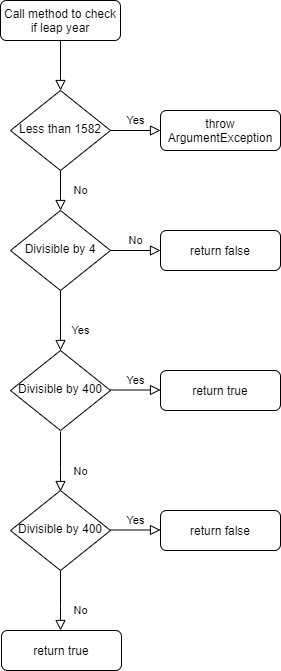
\includegraphics[height=\textheight]{leapyearalgorithm.png}
  \caption{Algorithm to check if a number represents a leap  year}
\end{figure}

\end{document}
